\documentclass[11pt]{article}

\usepackage[margin=1in]{geometry}
\usepackage{amsmath, amssymb, amsthm}
\usepackage{mathtools}
\usepackage{enumitem}
\usepackage{hyperref}
\usepackage{graphicx}
\usepackage{tikz}
\usetikzlibrary{arrows.meta, positioning, calc}
\usepackage{pgfplots}
\pgfplotsset{compat=1.18}

\newcommand{\HS}{H^\star}
\newcommand{\DN}{\Delta_N(u^{1:N};\gamma^{1:N})}
\newcommand{\JN}{J^N(\gamma^{0:N})}
\newcommand{\JNEE}{J^N_{EE}(\gamma^{0:N})}

\title{Critical Summary: Decentralized Detection with Many Sensors}
\author{Oren Ram \\ Ziv Abraham}
\date{\today}

\begin{document}
\maketitle

\section{Introduction - Decentralized Remote Hypothesis Testing}
In our critical summary, we discuss the results of the paper ``Decentralized Detection with Many Sensors: Optimality of Exchangeable and Identical Encoding Policies'' [1]. 
The paper addresses the problem of Decentralized Hypothesis Testing: many sensors observe an environment, compress their observations into actions, 
and send those actions to a fusion center (FC), which decides between two hypotheses, $H_1$ and $H_2$. While the paper's authors build 
tools for both the finite and infinite number of sensors regimes, in our work we focus on the 
finite-$N$ setting. %How to address asaf's note of n -> infty?

\section{Problem Setup}

Suppose there are two hypotheses, $H_1$ and $H_2$;
the true one is modeled as $\HS$, a random variable with $P(\HS = H_1) = p$, $P(\HS = H_2) = 1-p$. The system setup is:
\begin{itemize}
    \item $N < \infty$ sensors, each observing the environment and producing $y^i \in \mathcal{Y}^i$, the observation of the $i$-th sensor, for $i \in \{1,\dots, N\}$.
    \item Each sensor quantizes its observation using a mapping $\gamma^i: \mathcal{Y}^i \to \mathcal{U}^i$, where $\mathcal{U}^i$ denotes the set of actions the sensor can send.
    $\gamma^i$ is the decision rule / policy of the $i$-th sensor.
    \item The FC's policy is noted as $\gamma^0: \mathcal{U}^0 \times \mathcal{U}^1 \times \dots \times \mathcal{U}^N \to \{1,2\}$.\\
    Essentially, the fusion center decides $u^0 = \gamma^0(u^{1:N}), u^0 \in \{1,2\}$.\\
    Denote the set $\Gamma^i$ as the set of policies of sensor $i$, $\Gamma^0$ as the set of policies for the FC.
    \item The cost function we will focus on is:
    \begin{align}
        c(H_j,u^0)= 
                        \begin{cases}
                            1 & \text{if } u^0 \neq j \\
                            0 & \text{if } u^0 = j
                        \end{cases}
    \end{align}
    \item Our goal is to minimize the expected cost:
    \begin{align}
        J^N(\gamma^{0:N}) \triangleq \mathbb{E}^{\gamma^{0:N}}[c(H,u^{0:N})]
    \end{align}
\end{itemize}
\newpage
\subsection{Assumptions}
In order to make the problem tractable, the authors of the paper consider a few assumptions:
\begin{enumerate}[label=(\roman*)]
    \item $y^1, \dots, y^N$ are i.i.d. conditioned on $H$
    \item Under either hypothesis, sensor $i$'s observation has a probability density, measured against one common reference measure shared across both hypotheses.
    \item $\mathcal{U}^i = \mathcal{U}$ for $i = 1,\dots ,N$, and $\mathcal{U}$ is a finite set.
    \item The likelihood ratio:
    \begin{align}
        l^i = L(y^i) := \frac{f_{y^i|H}(y^i|H_2)}{f_{y^i|H}(y^i|H_1)} \text{ a.s.}
    \end{align}
    is well-behaved and invertible.
    \item Define $I_N^{KCR} \triangleq \{u^{1:N},\gamma^{1:N}\}$ to be the Known Common Randomization set, which includes all actions and policies of the sensors. We assume this set is known to the FC.
\end{enumerate}
While (i) is a common assumption in order to simplify the math and make it tractable, assumptions (ii) and (iv) are essential in order for $l^i$ to be a sufficient statistic of $y^i$, as will be discussed later.
Assumption (iii) dictates that all sensors have the same action set, an underlying assumption about the compression and rate being used. This will be discussed further in section *, where we will offer some modifications for the solution setup.
Assumption (v)'s essentiality will be discussed in Section~\ref{sec:threshold-map}.

\section{Sufficient Statistics, Existence of an Optimal Encoding Policy}

\subsection{Exponential Decay of the Error Probability}
\label{sec:exp-decay}
According to the law of large numbers, we can expect that $J^N(\gamma^{0:N})$ will
converge to the probability of error $P_e$ under decision rules $\gamma^{0:N}$. Also, under the criterion of minimizing the probability of error,
using the MAP rule at the fusion center is optimal for any sensor policy [2].\newline \newline
\textbf{[Proposition 5.1, 2]} - If $y^1,\dots,y^N$ are i.i.d. given $\HS$ and $P_{Y|H_1} \neq P_{Y|H_2}$, then there exists a decision rule $\gamma'$ and constants $\alpha, \beta > 0$ independent of $N$ such that
if all sensors use $\gamma'$ and the FC uses MAP then: $P_e < \alpha e^{-N\beta}$.\newline \newline
From [Proposition 5.1, 2], we can conclude that:

\begin{align}
     J^{N\star}(\gamma^{0:N}) = \inf_{\gamma^{0:N}}\{J^N(\gamma^{0:N})\} \leq J^{N}({\gamma'}^{0:N}) < \alpha e^{-N \beta} \label{eq:jnstar-bound}
\end{align}
From Equation~\eqref{eq:jnstar-bound} we can understand that $P_{e}$ of any relevant sequence of policies is exponentially decaying as $N$ grows large, hence we
need to study and optimize the \textbf{Error Exponent}, which characterizes how fast the error will decay given a sequence of policies. This leads to the definition:
\begin{equation}
    J_{EE}^{N}(\gamma^{0:N}) \triangleq -\frac{1}{N}\log(J^{N}(\gamma^{0:N})) \label{eq:error-exponent-def}
\end{equation}
We should notice that $J^{N}(\gamma^{0:N}) \le 1$ is a probability measure meaning its $\log$ is negative. By adding the negative sign, $J_{EE}^{N}(\gamma^{0:N})$ becomes a strictly positive rate. Hence, our goal is to maximize $J_{EE}^{N}(\gamma^{0:N})$ to achieve the fastest possible exponential decay of the error probability.
\subsection{$l^i$ is a Sufficient Statistic}
\label{sec:sufficient-statistic}
$l^i$ is a sufficient statistic of $H$: once its value is known, nothing else
about the raw observation $y^i$ can further move one's belief about which
hypothesis is true. With only two hypotheses under consideration, the entire way in which
the observation's density can vary with $H$ is exhausted by a single comparison --
how large the density is under $H_2$ relative to how large it is under $H_1$, at
that particular observation. A single number is therefore inherently enough to
hold everything that changes with $H$, and that number is, by construction,
exactly $l^i$. (How this shows up concretely inside the paper's own machinery --
via Lemma~1 -- is worth treating separately in a later section.)

\subsubsection*{No information loss: a Markov-chain and DPI reading}
Sufficiency means that any two raw observations producing the same $l^i$ are, for
the purpose of distinguishing $H_1$ from $H_2$, interchangeable: whatever detail of
$y^i$ is discarded in forming $l^i$ carries no evidential weight about $H$. This
has a clean information-theoretic statement. Since $l^i$ is a deterministic
function of $y^i$, the chain
\[
    H \;\to\; y^i \;\to\; l^i
\]
is trivially Markov, and the Data Processing Inequality (DPI) gives
\begin{equation}
    I(H; l^i) \le I(H; y^i).
\end{equation}
Equality holds \emph{iff} $l^i$ is sufficient for $H$ -- equivalently, iff
$H \to l^i \to y^i$ is \emph{also} a Markov chain, i.e.\ $y^i$ carries no further
information about $H$ once $l^i$ is fixed. This gives equality:
\begin{equation}
    I(H; l^i) = I(H; y^i).
\end{equation}
\subsection{Optimality of Threshold Policies and the MAP Decoder}
\label{sec:threshold-map}
\subsubsection*{Lemma 1}
For any fusion center decision rule $\gamma^0$,
\begin{equation}
    \inf_{\gamma^{1:N} \in \Gamma^N} J^N(\gamma^0, \gamma^{1:N})
    = \inf_{\gamma^{1:N} \in \Gamma^N_{TS}} J^N(\gamma^0, \gamma^{1:N}).
\end{equation}
where $\Gamma^N_{TS}$ is the class of threshold policies.

\smallskip
\noindent\textit{Why this reduction holds.} One direction is immediate: $\Gamma^N_{TS} \subseteq \Gamma^N$, so restricting the infimum to threshold policies can only raise it,
\begin{equation}
    \inf_{\gamma^{1:N} \in \Gamma^N} J^N(\gamma^0,\gamma^{1:N}) \;\le\; \inf_{\gamma^{1:N} \in \Gamma^N_{TS}} J^N(\gamma^0,\gamma^{1:N}).
\end{equation}
For the reverse direction, fix sensors $j \ne i$ to \emph{arbitrary} policies and ask what sensor $i$'s best response is. As shown below, this best response is always a threshold rule -- regardless of what the other $N-1$ sensors are doing, since the sub-problem sensor $i$ faces turns out to be linear in its own likelihood ratio $l^i$. Because this holds for any fixed configuration of the rest, we can replace each sensor's policy, one at a time, with its threshold best-response: the cost $J^N$ never increases at any step. After $N$ such replacements every sensor uses a threshold rule, and the resulting cost is no larger than that of the original arbitrary profile. Taking the infimum over the starting profile gives
\begin{equation}
    \inf_{\gamma^{1:N} \in \Gamma^N_{TS}} J^N(\gamma^0,\gamma^{1:N}) \;\le\; \inf_{\gamma^{1:N} \in \Gamma^N} J^N(\gamma^0,\gamma^{1:N}),
\end{equation}
and combined with the trivial direction, equality holds. This is the standard \emph{person-by-person optimization} argument: joint optimality follows from unilateral optimality of each coordinate, holding all others fixed.

\smallskip
\noindent Concretely, fixing every sensor's policy except sensor $i$'s, sensor $i$'s optimization is:
\begin{align}
    \inf_{u^i \in \mathcal U} \bigg\{\sum_{j=1,2} P(H_j \mid y^i)\, E_{\gamma^{-i\star}}\big[c(H_j, \gamma^0(u^{1:N})) \mid H_j\big]\bigg\}
\end{align}

By Bayes' rule,
\begin{equation}
    P(H_j \mid y^i) = \frac{f_{y^i|H}(y^i \mid H_j)\,P(H_j)}{f_{y^i}(y^i)}, \qquad j=1,2,
\end{equation}
and taking the ratio of the two, the normalizer $f_{y^i}(y^i)$ cancels:
\begin{equation}
    \frac{P(H_2 \mid y^i)}{P(H_1\mid y^i)} = \frac{f_{y^i|H}(y^i\mid H_2)}{f_{y^i|H}(y^i\mid H_1)}\cdot\frac{P(H_2)}{P(H_1)} = l^i \cdot \frac{P(H_2)}{P(H_1)}.
\end{equation}
So the ratio of posteriors -- all that matters for comparing the two terms in the sum above -- depends on $y^i$ only through the likelihood ratio $l^i$: exactly the sufficiency of $l^i$ from Section~\ref{sec:sufficient-statistic}, showing up again inside the optimization itself.

Writing $g^i(H_j,u^i) \triangleq E_{\gamma^{-i\star}}[c(H_j,\gamma^0(u^{1:N}))\mid H_j]$ for the expected cost of action $u^i$ under $H_j$ given the other sensors' fixed policies, and factoring the positive term $P(H_1\mid y^i)$ out of the sum (it does not affect the $\arg\inf$),
\begin{equation}
    \sum_{j=1,2} P(H_j\mid y^i)\,g^i(H_j,u^i) = P(H_1\mid y^i)\left[g^i(H_1,u^i) + \frac{P(H_2\mid y^i)}{P(H_1\mid y^i)}\,g^i(H_2,u^i)\right].
\end{equation}
Dropping the positive prefactor $P(H_1\mid y^i)$ and substituting the ratio derived above, the sub-problem reduces to
\begin{equation}
    \inf_{u^i \in \mathcal U} \left[ g^i(H_1, u^i) + g^i(H_2, u^i)\, l^i\,
    \frac{P(H_2)}{P(H_1)} \right].
\end{equation}
This is linear in $l^i$ for each action, so the best action is whichever line is lowest at that value of $l^i$, switching only at the points where lines cross -- a threshold rule.
\subsubsection*{Lemma 2}
Under the assumptions above, for any deterministic encoding policy of the sensors, the optimal policy of the fusion center is given by:
\begin{align}
    \gamma^{0\star}(u^{1:N}) =                         
        \begin{cases}
            H_1 & \text{if }    \Delta_N(u^{1:N};\gamma^{1:N}) \geq t \\
            H_2 & \text{if }      \Delta_N(u^{1:N};\gamma^{1:N}) < t
        \end{cases}
\end{align}
for some $t \in \mathbb{R}$ and $\DN$ given by:
\begin{align}
    \DN \triangleq \frac{1}{N}\sum_{i=1}^{N}\log \frac{P^{\gamma^i}(u^i|H_1)}{P^{\gamma^i}(u^i|H_2)}
\end{align}
Recalling that in [2] it was established that the MAP rule is optimal for any deterministic sensor policy.
The MAP rule for our problem is:
\begin{align}
    \gamma^{0\star}(u^{1:N}) = \arg\max_{i \in \{1,2\}}P(H_i|u^{1:N})
\end{align}
It can be written in the form of a log likelihood decision rule:
\begin{align}
    \gamma^{0\star}(u^{1:N}) =
    \begin{cases}
        H_1 & \text{if }        \log \frac{P(H_1|u^{1:N})}{P(H_2|u^{1:N})} \geq 0\\
        H_2 & \text{if }        \log \frac{P(H_1|u^{1:N})}{P(H_2|u^{1:N})} < 0
    \end{cases}
\end{align}
And looking at the log likelihood:
\begin{align}
    \log \frac{P(H_1|u^{1:N})}{P(H_2|u^{1:N})} &= \log \frac{P(u^{1:N}|H_1)}{P(u^{1:N}|H_2)} + \log\frac{P(H_1)}{P(H_2)} \label{eq:bayes-step}\\
    &= \log \prod _{i = 1}^{N} \frac{P^{\gamma^i}(u^i|H_1)}{P^{\gamma^i}(u^i|H_2)} + \underbrace{\log\frac{p}{1-p}}_{\triangleq -Nt} \label{eq:iid-step}\\
    &= \sum_{i=1}^{N}\log\frac{P^{\gamma^i}(u^i|H_1)}{P^{\gamma^i}(u^i|H_2)} - Nt
\end{align}
Here, Equation~\eqref{eq:bayes-step} follows from Bayes' rule, and Equation~\eqref{eq:iid-step} from $y^i$ being i.i.d. given $H$. We should just note that:
\begin{align}
    \sum_{i=1}^{N}\log\frac{P^{\gamma^i}(u^i|H_1)}{P^{\gamma^i}(u^i|H_2)} - Nt \geq 0 \iff \frac{1}{N}\sum_{i=1}^{N}\log\frac{P^{\gamma^i}(u^i|H_1)}{P^{\gamma^i}(u^i|H_2)} \geq t
\end{align}
And this sums up how the optimal decision rule of the FC is established. It is important to note that this decision rule is why assumption (v) is important for the paper's solution:
in order to calculate $\DN$, the FC must know how $u^i$ was derived, to give it its proper weight in the decision process.
\subsection{Existence of an Optimal Solution}
Lemmas 1 and 2 characterize the necessary structure of an optimal policy -- threshold at the sensors, MAP at the FC. Theorem 1, using the compactness result of Lemma 3, establishes that a minimizer with this structure exists.
\subsubsection*{Lemma 3}
\begin{center}
    $\Gamma^N_{TS}$ is compact under total variation.
\end{center}
Lemma 3 is an important step towards establishing the \textbf{existence} of an optimal solution, the paper's main contribution to the finite $N$ problem.

\subsubsection*{Theorem 1}
There exists an optimal decision rule sequence $\gamma^{0:N\star} = (\gamma^{0\star},\gamma^{1\star},\dots, \gamma^{N\star})$. These policies are MAP for the FC and threshold for the sensors.\\
The proof of Theorem 1 follows from Lemmas 1 and 2, together with the compactness of $\Gamma^N_{TS}$ (Lemma 3). Since $J^N(\gamma^{0:N})$ is continuous in the sensors' policies over this compact set, Weierstrass's extreme value theorem guarantees that the infimum is attained.

\section{Calculating the error exponent}
\label{sec:error-exponent}
Under assumptions (i) - (v) and Theorem 1, we can formulate a closed-form bound for the error exponent. 
Bounding each of the two error events with a Chernoff bound, in terms of a policy-dependent Chernoff coefficient 
$M(\alpha,\gamma^i)$, and combining them gives a bound on $P_e$. Taking $-\frac{1}{N}\log(\cdot)$ of this bound and letting $N \to \infty$ yields, 
for $K$ distinct policies used by fractions $c_k$ of the sensors:
\begin{align}
    \lim_{N \to \infty}\JNEE \geq -\min_{\alpha \in [0,1]}\sum_{k=1}^{K} c_k \log M(\alpha,\gamma^k) \label{eq:error-exponent-bound}
\end{align}
Where
\begin{align}
    M(\alpha,\gamma^i) \triangleq \sum_{u \in \mathcal{U}} P^{\gamma^i}(u^i|H_2)^{1-\alpha}P^{\gamma^i}(u^i|H_1)^{\alpha}
\end{align}
The full derivation is given in Appendix~\ref{app:error-exponent}.\newline
We can use the bound in Equation~\eqref{eq:error-exponent-bound} to get a closed form bound of the exponent in Equation~\eqref{eq:jnstar-bound}. Assuming all the sensors policies are identical,
$K = 1, c_1 = 1$ and we get the definition of \textbf{Chernoff Distance} [3]:
\begin{align*}
    \lim_{N \to \infty}\JNEE \geq -\min_{\alpha \in [0,1]}\log M(\alpha,\gamma) = C(P^\gamma_{Y|H_1},P^\gamma_{Y|H_2})
\end{align*}
\subsection*{Discussion of the result}
\begin{align}
    C(P^\gamma_{Y|H_1},P^\gamma_{Y|H_2}) = -\min_{\alpha \in [0,1]}\log\bigg(\sum_{u \in \mathcal{U}} P^{\gamma}(u^i|H_2)^{1-\alpha}P^{\gamma}(u^i|H_1)^{\alpha}\bigg) \label{eq:chernoff-distance}
\end{align}
As defined in [3], the Chernoff distance (Chernoff information) is a measure of \textbf{distinguishability} between two probability distributions;\newline
If $P(u^i|H_1) = 1$, the hypotheses are perfectly distinguishable, so $P(u^i|H_2) = 0$: the sum inside the logarithm vanishes, the error exponent diverges, and $P_e \to 0$.\newline
On the other hand, if $P(u^i|H_1) = P(u^i|H_2)$ for all $u \in \mathcal{U}$, the hypotheses are indistinguishable: the sum equals 1, the error exponent vanishes, and $P_e$ fails to decay.\newline
For any other conditional probabilities, the Chernoff distance provides a solid bound on the error exponent.\newline
This result is highly intuitive: as the quantized observations under each hypothesis become more distinguishable, the Chernoff distance grows. This yields a larger error exponent, which drives a steeper exponential decay in the probability of error. In practical terms, greater distinguishability at the sensor level guarantees an exponentially better detection performance as the number of sensors grows.
\newpage

\section{Considering rate}
\label{sec:considering-rate}
We now turn to the total rate consumed by the sensors. We consider two encoding and transmission policies. 
The first is the \textbf{vanilla} policy, under which every sensor transmits its action using $R$ bits regardless of how confident it is in that decision.
The second is a \textbf{silent} policy, in which we introduce two thresholds on each sensor's decision rule: a sensor transmits its action using $R$ bits only if its observation falls outside of a silent bin, meaning it is "confident" in its decision.
\subsection*{Assumptions}
\begin{itemize}
    \item Assumptions (i) to (v) hold.
    \item Gaussian model - $y^i|H_1 \sim \mathcal{N}(0,\sigma^2)$ and $y^i|H_2 \sim \mathcal{N}(\mu,\sigma^2)$
        \begin{figure}[h!]
            \centering
            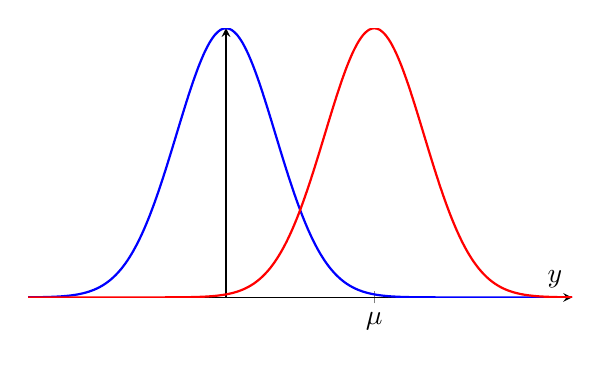
\begin{tikzpicture}
                \begin{axis}[
                    width=0.7\textwidth,
                    height=5cm,
                    axis lines = middle,
                    xlabel = {$y$},
                    xtick = {0, 3},
                    xticklabels = {$0$, $\mu$},
                    ytick = \empty,
                    samples = 100,
                    domain = -4:7,
                ]
                \addplot[thick, blue, smooth] {1/sqrt(2*pi)*exp(-x^2/2)};
                \addplot[thick, red, smooth] {1/sqrt(2*pi)*exp(-(x-3)^2/2)};
                \end{axis}
            \end{tikzpicture}
        \end{figure}
    \item Each sensor can send up to $R$ bits to the fusion center, meaning $\mathcal{U} = \{u^1,\dots, u^{2^R}\}$.
    \item All sensors use the same policy - $\gamma^V$ for the Vanilla setup and $\gamma^S$ for the silent setup.
\end{itemize}
For each setup, we derive the corresponding Chernoff distance bound of Equation~\eqref{eq:chernoff-distance} and evaluate the setups' performance via simulation.


\subsubsection*{General $R$-bit Threshold Policy}
 
We generalize Setup A and Setup B into a single family of threshold
policies, indexed by the number of bits $R$, a bin width $\Delta>0$, and
a silence half-width $\delta \ge 0$.
 
Let $L \triangleq 2^R$ and $\mathcal{U} = \{u^1,\dots,u^L,u^S\}$, where
$u^S$ denotes silence. For $\delta \ge 0$, define the thresholds
\begin{equation}
t_j(\delta) \triangleq
\begin{cases}
\dfrac{\mu}{2} - \delta - \Big(\dfrac{L}{2}-j\Big)\Delta, & j = 1,\dots,\dfrac{L}{2} \\[2mm]
\dfrac{\mu}{2} + \delta + \Big(j-\dfrac{L}{2}-1\Big)\Delta, & j = \dfrac{L}{2}+1,\dots,L
\end{cases},
\qquad t_0 \triangleq -\infty, \quad t_{L+1} \triangleq +\infty.
\label{eq:general-thresholds}
\end{equation}
The policy $\gamma^R_{\Delta,\delta}$ sends $u^m$ if $y \in (t_{m-1},t_m)$
for $m=1,\dots,L/2$, stays silent if $y \in (t_{L/2},t_{L/2+1})$, and
sends $u^m$ if $y \in (t_m,t_{m+1})$ for $m=L/2+1,\dots,L$.
 
At $\delta=0$, $t_{L/2}=t_{L/2+1}=\mu/2$: the silence interval degenerates
to a point, $u^S$ is never sent, and $\gamma^R_{\Delta,0}$ is an
$L$-region always-transmit policy. We define
\begin{equation}
\gamma^V \triangleq \gamma^R_{\Delta,0}, \qquad
\gamma^S \triangleq \gamma^R_{\Delta,\delta}, \ \ \delta > 0.
\label{eq:vanilla-silent-def}
\end{equation}
 
% \begin{figure}[h]
%   \centering
%   % TODO: generalized version of Figures 2/3 (Section 5) and Figures
%   % 4/5 (Simulation Plan): L thresholds, L/2 bins per side, silence
%   % bin of half-width delta shrinking to a point as delta -> 0.
%   \caption{Gaussian model for the general $R$-bit threshold policy $\gamma^R_{\Delta,\delta}$.}
% \end{figure}
 
Standardizing by $\sigma$,
\begin{equation}
a_j \triangleq \frac{t_j(\delta)}{\sigma}, \qquad
c_j \triangleq \frac{t_j(\delta)-\mu}{\sigma} = a_j - s, \qquad
s \triangleq \frac{\mu}{\sigma}, \qquad
a_0 = c_0 \triangleq -\infty, \quad a_{L+1}=c_{L+1}\triangleq+\infty.
\label{eq:general-standardized}
\end{equation}
Every quantity below is written in terms of $a_j,c_j$ and applies to
$\gamma^V$ and $\gamma^S$ alike.
 
\subsubsection*{Symbol Probabilities}

Since $L(y)$ is increasing in $y$ (Appendix~\ref{app:vanilla-derivation}),
each region's probability under the Gaussian model is a difference of
$Q$-functions. For the left-hand symbols $m = 1,\dots,L/2$,
\begin{align}
P^{\gamma^R_{\Delta,\delta}}(u^m\mid H_1) &= Q(a_{m-1}) - Q(a_m), &
P^{\gamma^R_{\Delta,\delta}}(u^m\mid H_2) &= Q(c_{m-1}) - Q(c_m),
\label{eq:prob-left}
\end{align}
for the silence symbol,
\begin{align}
P^{\gamma^R_{\Delta,\delta}}(u^S\mid H_1) &= Q(a_{L/2}) - Q(a_{L/2+1}), &
P^{\gamma^R_{\Delta,\delta}}(u^S\mid H_2) &= Q(c_{L/2}) - Q(c_{L/2+1}),
\label{eq:prob-silence}
\end{align}
and for the right-hand symbols $m = L/2+1,\dots,L$,
\begin{align}
P^{\gamma^R_{\Delta,\delta}}(u^m\mid H_1) &= Q(a_m) - Q(a_{m+1}), &
P^{\gamma^R_{\Delta,\delta}}(u^m\mid H_2) &= Q(c_m) - Q(c_{m+1}).
\label{eq:prob-right}
\end{align}
 
\subsubsection*{Threshold Symmetry}
 
The thresholds \eqref{eq:general-thresholds} satisfy, for every
$j=0,\dots,L+1$,
\begin{equation}
t_{L+1-j}(\delta) = \mu - t_j(\delta), \qquad \text{equivalently} \qquad
a_{L+1-j} = s - a_j, \quad c_{L+1-j} = -a_j.
\label{eq:mirror-thresholds}
\end{equation}
Together with $f_{y\mid H_1}(y) = f_{y\mid H_2}(\mu-y)$,
Eq.~\eqref{eq:mirror-thresholds} gives
\begin{equation}
P^{\gamma^R_{\Delta,\delta}}(u^m\mid H_1) = P^{\gamma^R_{\Delta,\delta}}(u^{L+1-m}\mid H_2),
\qquad m=1,\dots,L,
\label{eq:mirror-probs}
\end{equation}
and the silence probability is hypothesis-independent,
\begin{equation}
P^{\gamma^R_{\Delta,\delta}}(u^S\mid H_1) = P^{\gamma^R_{\Delta,\delta}}(u^S\mid H_2)
\triangleq P^{\gamma^R_{\Delta,\delta}}(u^S)
= Q\Big(\frac{s}{2}-\frac{\delta}{\sigma}\Big) - Q\Big(\frac{s}{2}+\frac{\delta}{\sigma}\Big).
\label{eq:silence-prob}
\end{equation}
 
\subsubsection*{Chernoff Coefficient}
 
Generalizing Equation (25) to $L+1$ symbols,
\begin{equation}
M(\alpha; R,\Delta,\delta) \triangleq P^{\gamma^R_{\Delta,\delta}}(u^S)
+ \sum_{m=1}^{L} P^{\gamma^R_{\Delta,\delta}}(u^m\mid H_2)^{1-\alpha}\,
P^{\gamma^R_{\Delta,\delta}}(u^m\mid H_1)^{\alpha}.
\label{eq:chernoff-general}
\end{equation}
By Equation (24) with $K=1$,
\begin{equation}
\lim_{N\to\infty} J_{EE}^N(\gamma^{0:N}) \ge
-\min_{\alpha\in[0,1]} \log M(\alpha; R,\Delta,\delta).
\label{eq:general-bound-alpha}
\end{equation}
 
Substituting $m \to L+1-m$ and using
Eqs.~\eqref{eq:mirror-probs}-\eqref{eq:silence-prob} gives
$M(1-\alpha;R,\Delta,\delta) = M(\alpha;R,\Delta,\delta)$. Each summand in
\eqref{eq:chernoff-general} is convex in $\alpha$, so
$M(\cdot;R,\Delta,\delta)$ is convex on $[0,1]$; symmetry about
$\alpha=0.5$ then places its minimum there, as in Equations (27) and (29).
 
\subsubsection*{Closed-Form Bound}

\begin{align}
C(R,\Delta,\delta) &\triangleq -\log M(0.5; R,\Delta,\delta) \nonumber \\
&= -\log\left[P^{\gamma^R_{\Delta,\delta}}(u^S)
+ \sum_{m=1}^{L} \sqrt{P^{\gamma^R_{\Delta,\delta}}(u^m\mid H_1)\,
P^{\gamma^R_{\Delta,\delta}}(u^m\mid H_2)}\right],
\label{eq:general-closed-form}
\end{align}
\begin{equation}
\lim_{N\to\infty} J_{EE}^N(\gamma^{0:N}) \ge C(R,\Delta,\delta).
\label{eq:general-closed-form-bound}
\end{equation}
 
\subsubsection*{Recovering Setup A and Setup B}
 
Define $C_V(R,\Delta) \triangleq C(R,\Delta,0)$ and, for $\delta>0$,
$C_S(R,\Delta,\delta) \triangleq C(R,\Delta,\delta)$.
 
At $\delta=0$, $a_{L/2}=a_{L/2+1}=s/2$, so $P^{\gamma^V}(u^S)=0$ and
\eqref{eq:general-closed-form} reduces to the $L$-region vanilla bound.
At $R=1$ ($L=2$), $a_1 = s/2 \mp \delta/\sigma$ does not depend on
$\Delta$, and \eqref{eq:general-closed-form} reduces to Equation (28) at
$\delta=0$ and to Equation (30) at $\delta>0$, recovering the one-bit
case exactly.

\subsubsection*{The Unquantized Ceiling}

Before evaluating the bound it is worth fixing what it is bounded by.
Suppose the sensor forwards $y^i$ itself, at infinite precision. Under the
Gaussian model
\begin{equation}
M_\infty(\alpha) \triangleq \int f_{y|H_2}^{1-\alpha}(y)\,f_{y|H_1}^{\alpha}(y)\,dy
= \exp\!\Big(-\alpha(1-\alpha)\tfrac{\mu^2}{2\sigma^2}\Big),
\label{eq:M-infty}
\end{equation}
which is again symmetric about $\alpha=1/2$ and convex, so the minimum sits
there as in Equation~\eqref{eq:general-closed-form}, giving
\begin{equation}
C_\infty \triangleq -\min_{\alpha\in[0,1]}\log M_\infty(\alpha)
= \frac{\mu^2}{8\sigma^2} = \frac{s^2}{8}.
\label{eq:ceiling}
\end{equation}
Since $H \to y^i \to u^i$ is Markov for any policy, the Data Processing
Inequality of Section~\ref{sec:sufficient-statistic} applies to $\gamma$ as
it did to $l^i$: quantization can discard evidence about $H$, never create
it. Hence
\begin{equation}
C(R,\Delta,\delta) \le C_\infty \qquad \text{for every } R,\Delta,\delta,
\label{eq:ceiling-bound}
\end{equation}
and $C_\infty$ is the natural yardstick against which every finite-rate
policy is measured. Note that $C_\infty$ depends on the model only through
$s = \mu/\sigma$: the whole problem is how many standard deviations apart
the two hypotheses sit.

\subsubsection*{Transmitted Rate}

The parameter $R$ is the rate $\gamma^V$ pays, but not the rate $\gamma^S$
pays: a silent sensor sends nothing. Using
Equation~\eqref{eq:silence-prob}, the expected transmitted rate is
\begin{equation}
\bar R(R,\Delta,\delta) \triangleq R\,\Big(1 - P^{\gamma^R_{\Delta,\delta}}(u^S)\Big),
\label{eq:mean-rate}
\end{equation}
so $\bar R = R$ for $\gamma^V$ and $\bar R < R$ for $\gamma^S$. Comparisons
made at equal $R$ therefore charge $\gamma^S$ for bandwidth it never uses.

\subsection*{Simulation Results}
\label{sec:sim-results}

We evaluate $\gamma^R_{\Delta,\delta}$ for $R = 1,\dots,5$ at
$N = 3000$ sensors and $p = \tfrac12$, at three operating points
$\mathrm{SNR} \in \{-5, 0, +5\}$~dB. At each point $(\Delta^\star,
\delta^\star)$ are chosen to maximize the closed-form bound
$C(R,\Delta,\delta)$ of Equation~\eqref{eq:general-closed-form}; Setup A
pins $\delta = 0$, so $\gamma^V$ optimizes over $\Delta$ alone. The
fusion center computes $J^N$ exactly, from which $J^N_{EE}$ follows by
Equation~\eqref{eq:error-exponent-def}.

% TODO: regenerate these three panels with the C_infty ceiling line and the
% C(R, Delta*, delta*) bound curves overlaid (Figs/fig_JEE_vs_R_N3000_*.png).
\begin{figure}[h!]
    \centering
    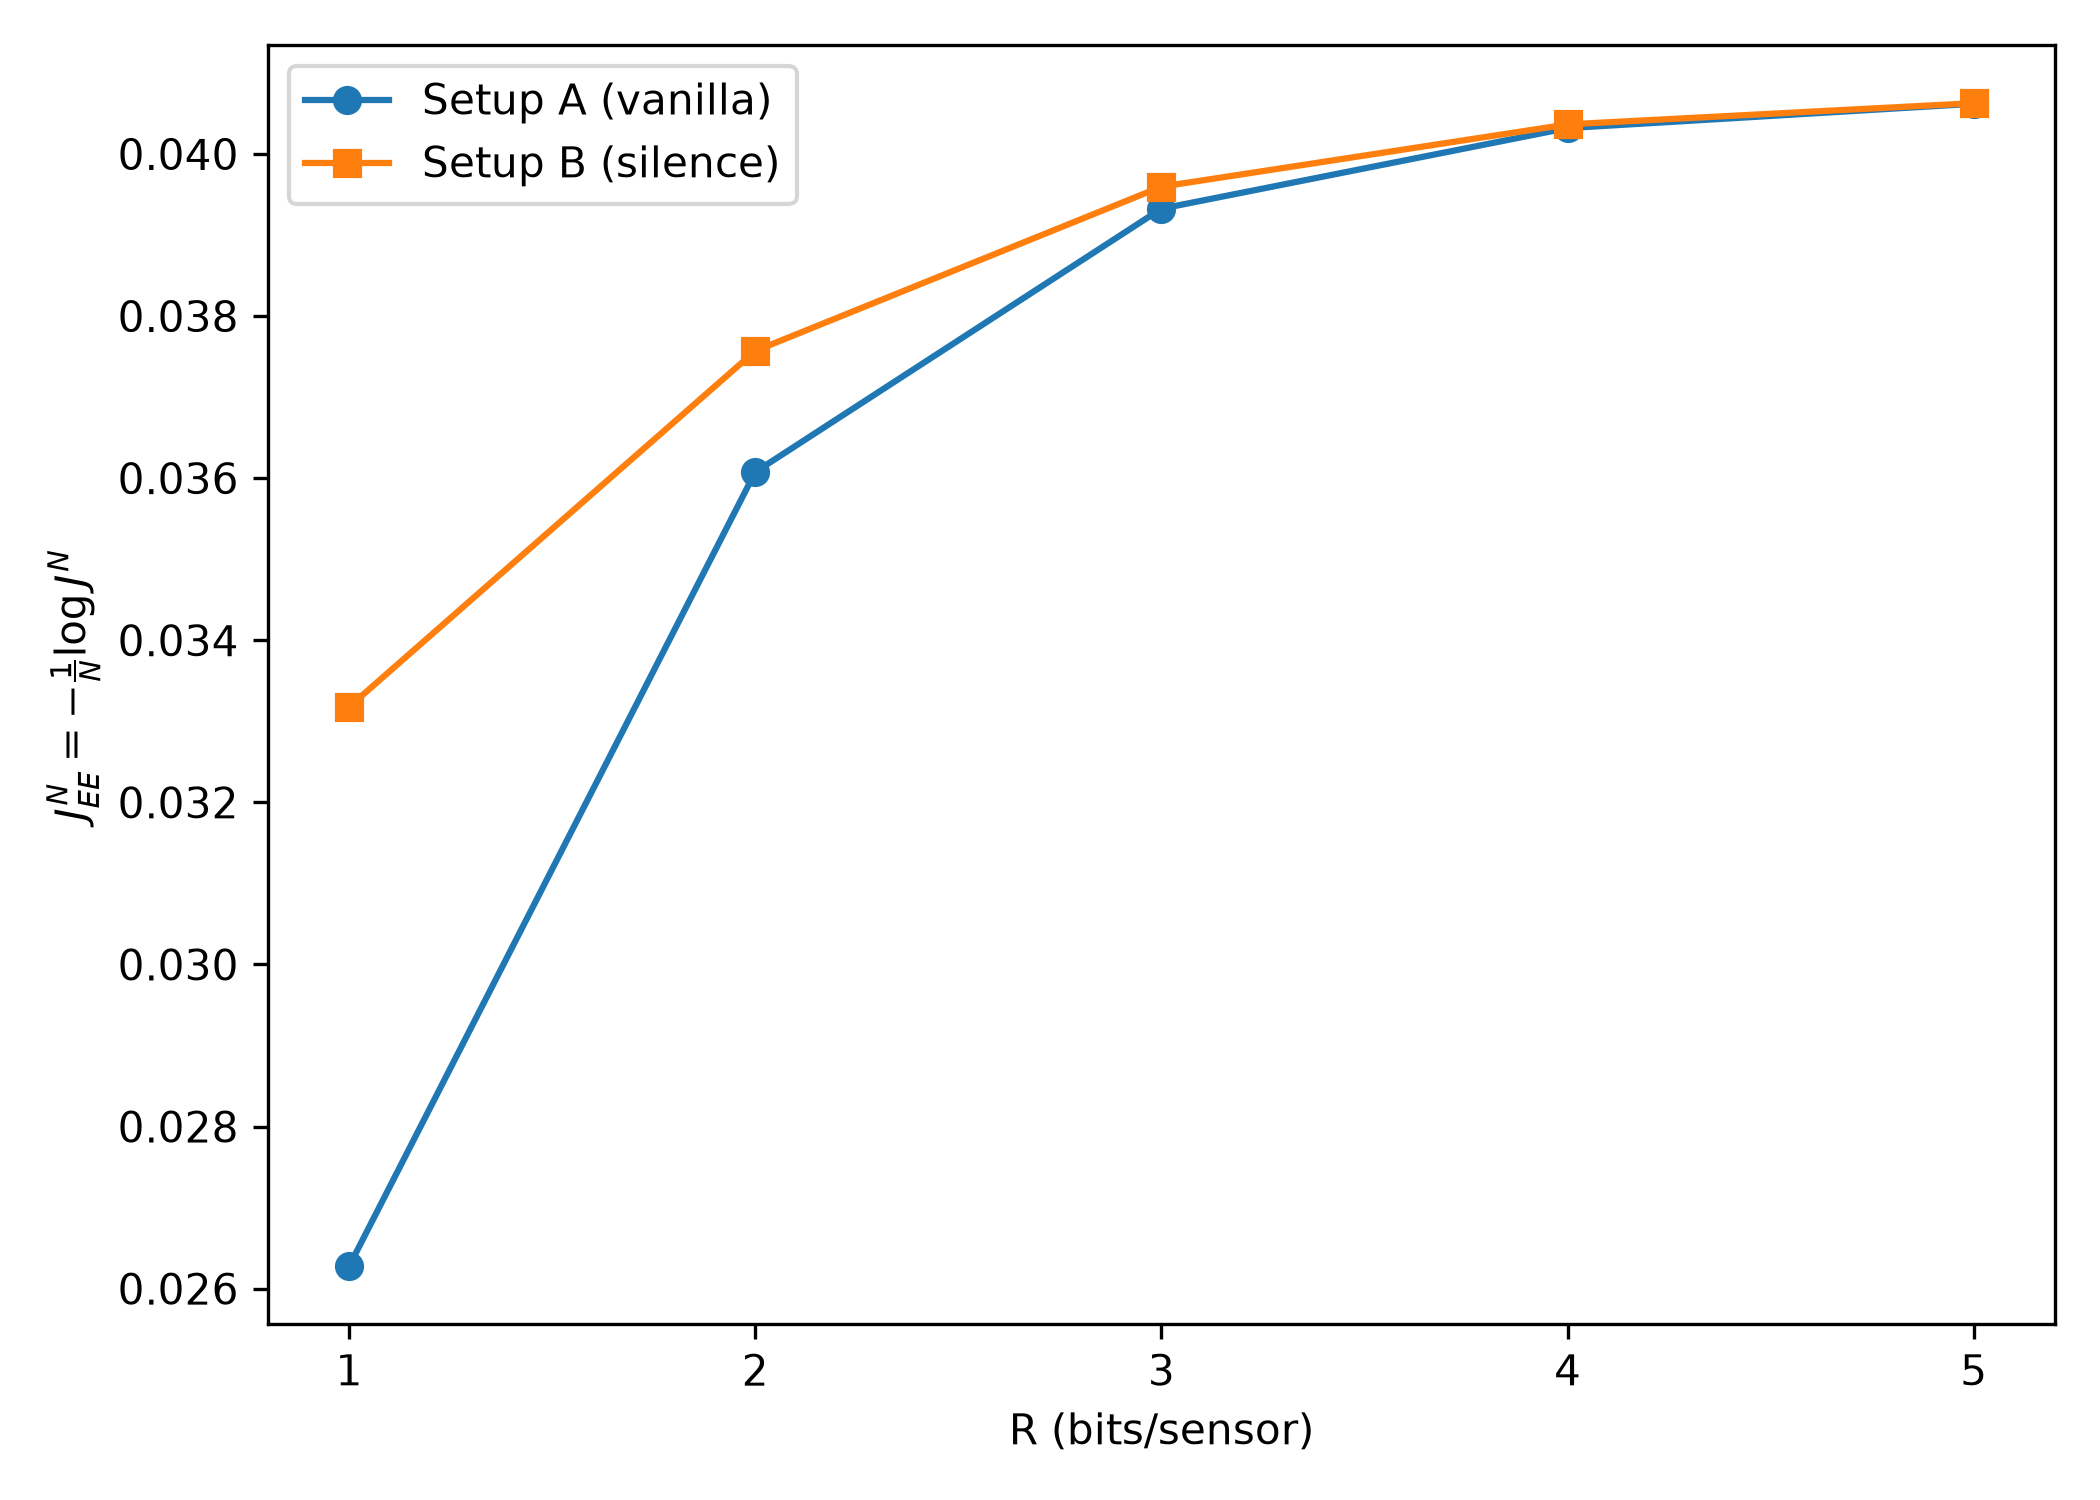
\includegraphics[width=0.32\textwidth]{Figs/fig_JEE_vs_R_N3000_snrm5.png}
    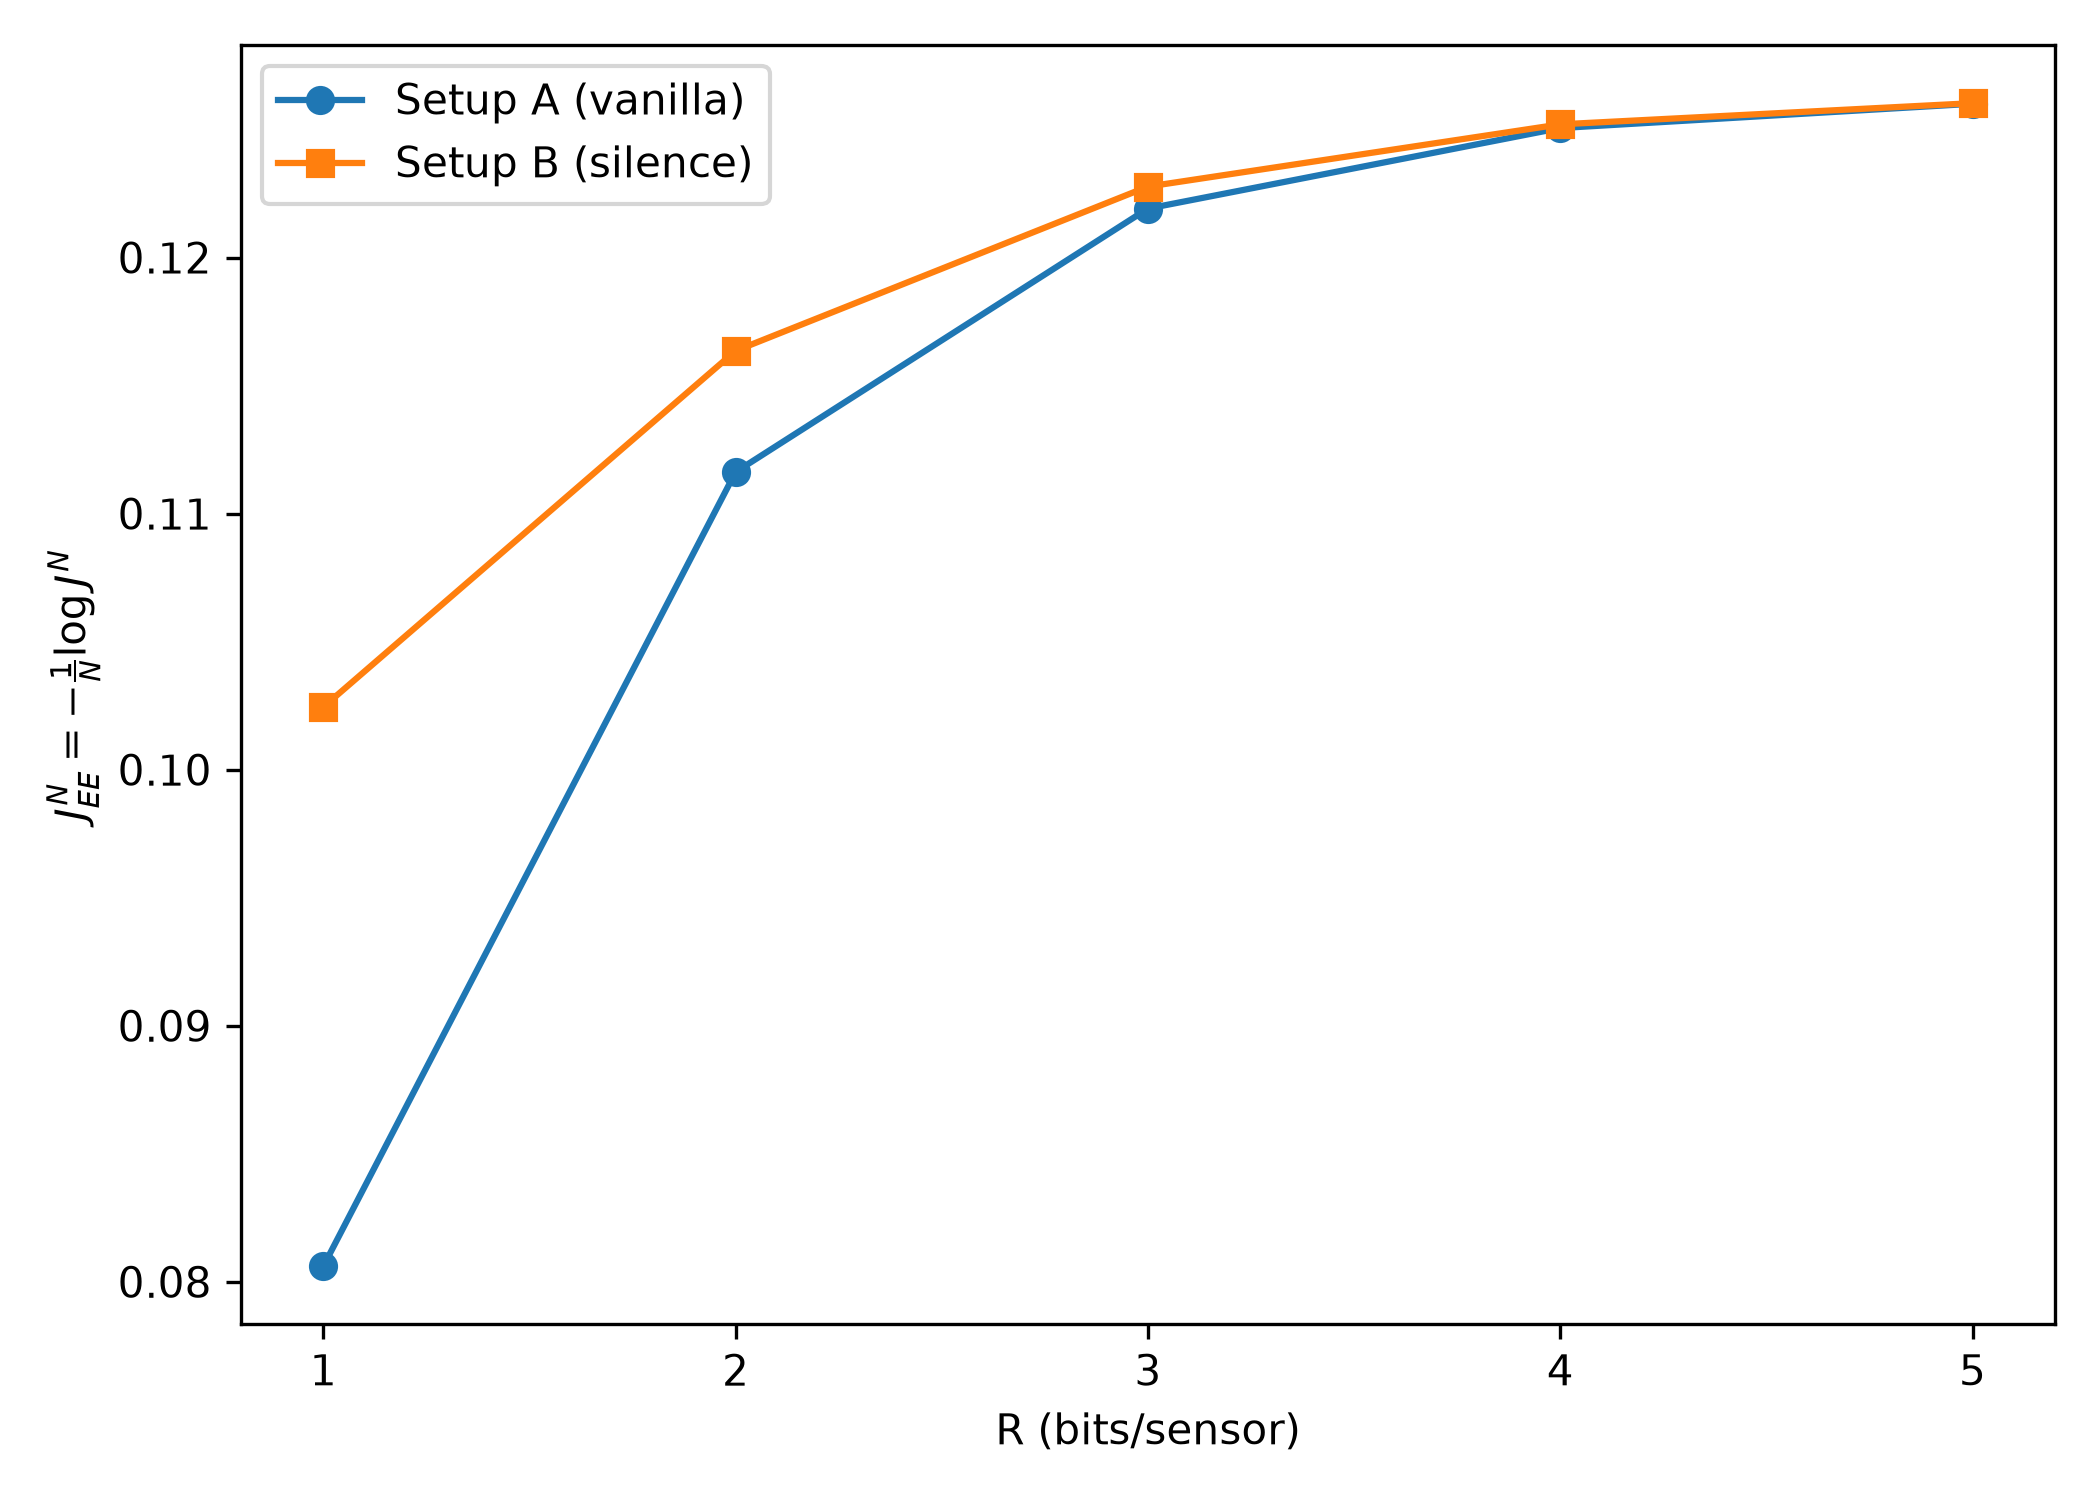
\includegraphics[width=0.32\textwidth]{Figs/fig_JEE_vs_R_N3000_snrp0.png}
    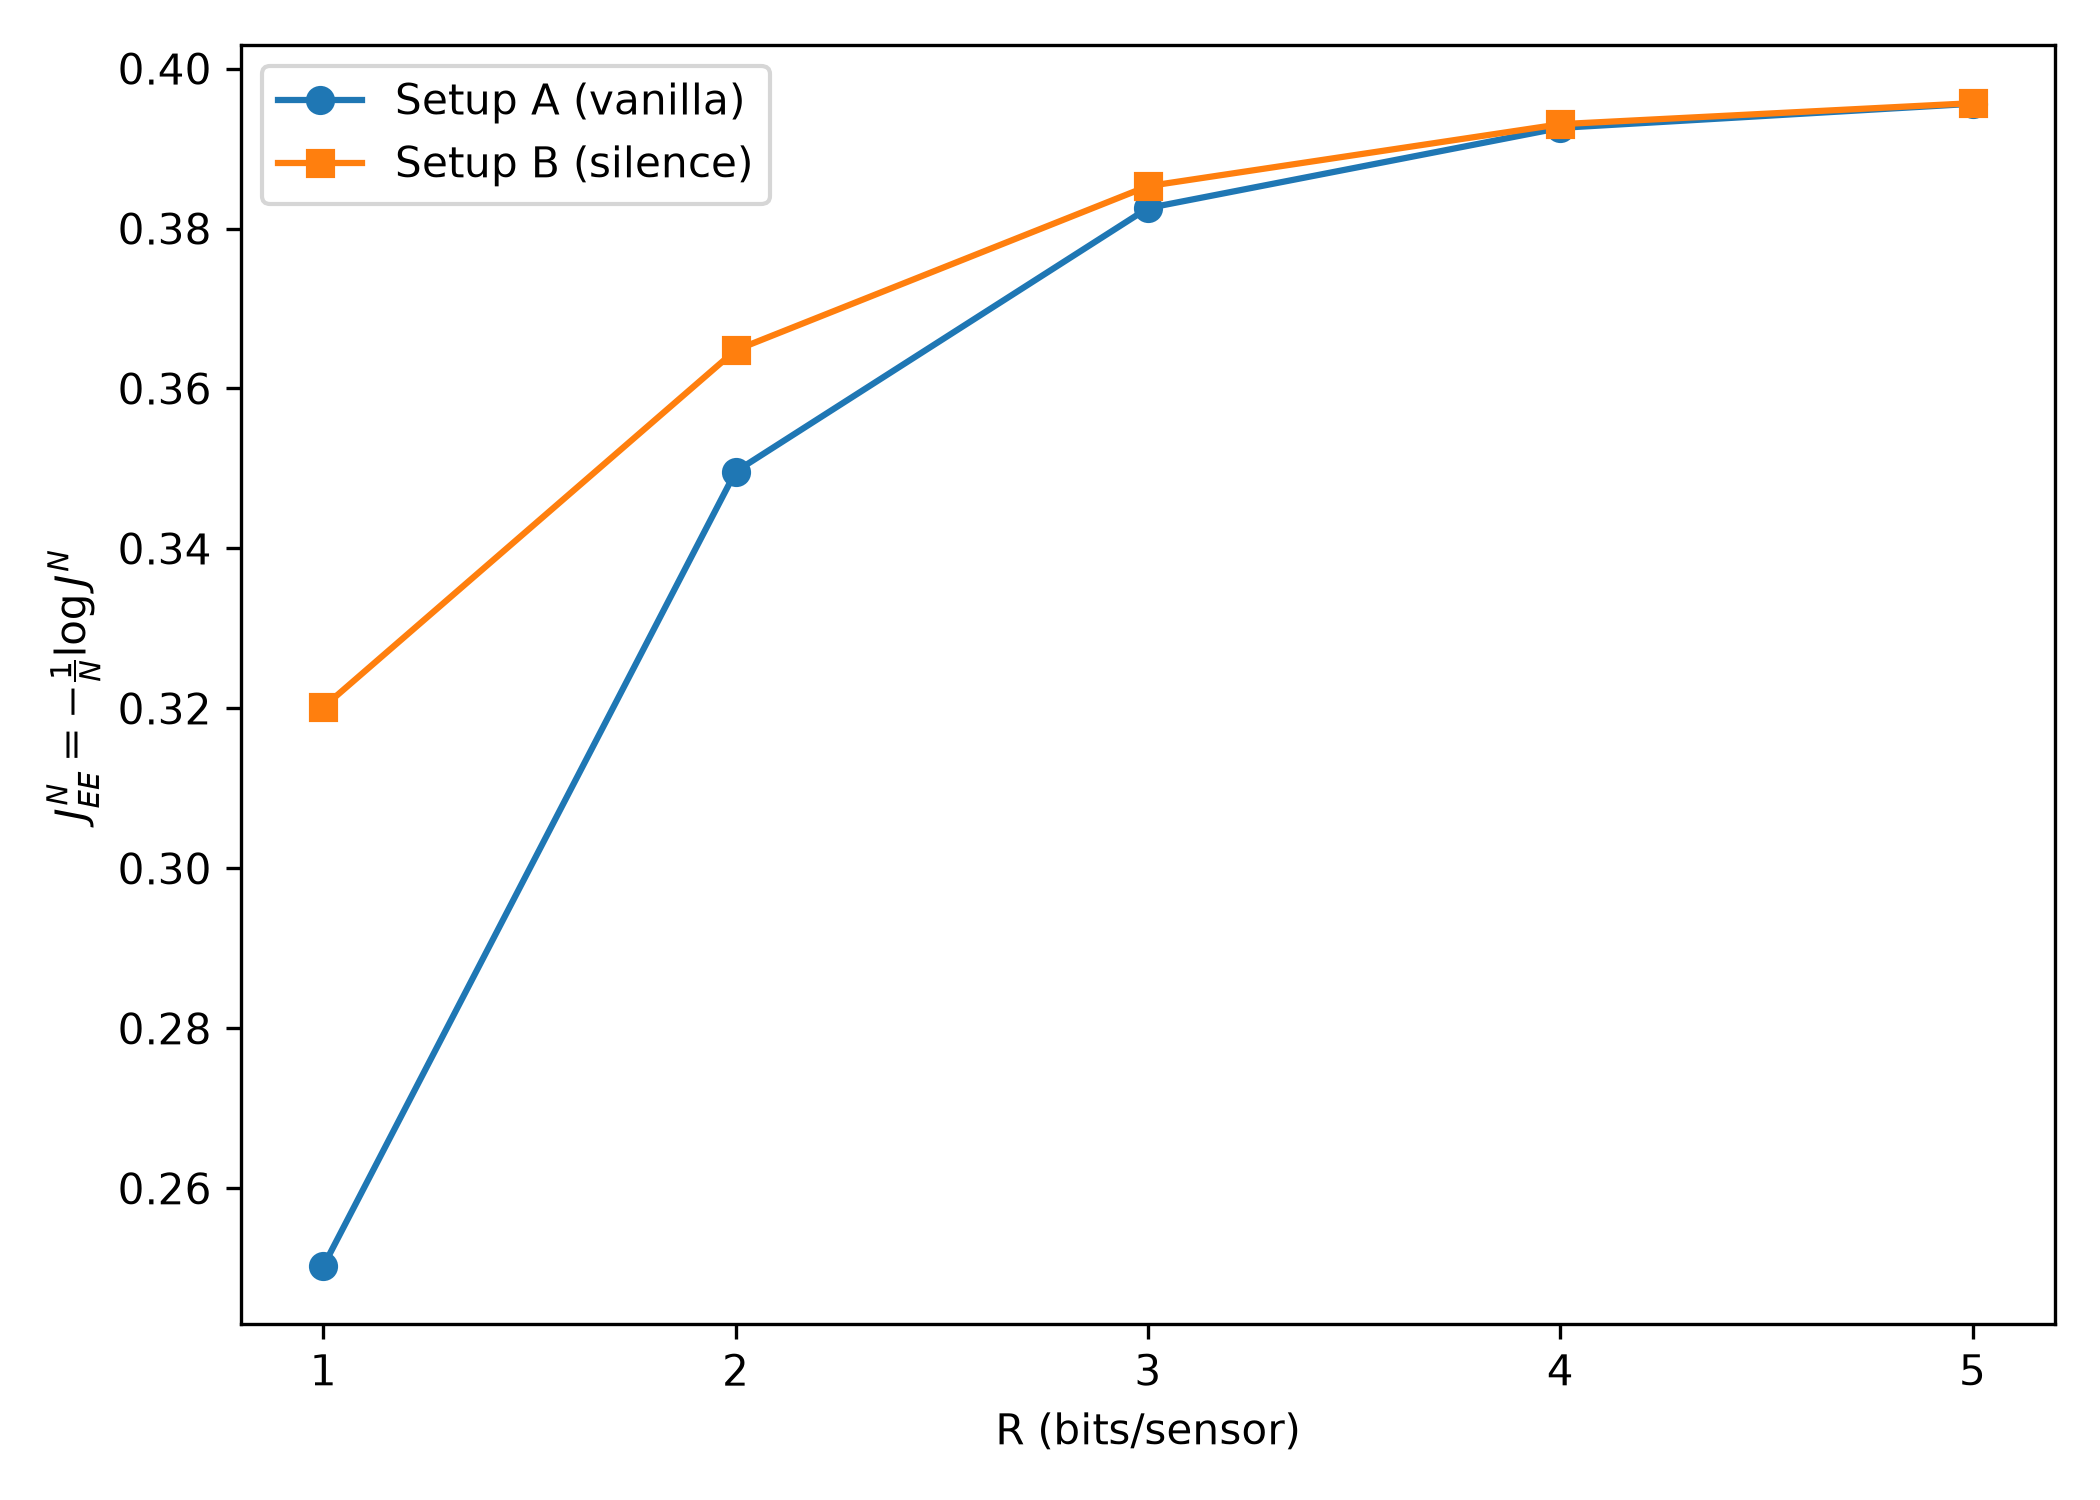
\includegraphics[width=0.32\textwidth]{Figs/fig_JEE_vs_R_N3000_snrp5.png}
    \caption{Normalized error exponent $J^N_{EE}$ against $R$ at the optimal
    $(\Delta^\star,\delta^\star)$, for $N = 3000$ and
    $\mathrm{SNR} = -5, 0, +5$~dB (left to right). Setup A is
    $\gamma^V$, Setup B is $\gamma^S$.}
    \label{fig:jee-vs-R}
\end{figure}

Figure~\ref{fig:jee-vs-R} shows one shape repeated at all three operating
points. $J^N_{EE}$ rises monotonically in $R$ and saturates onto the
unquantized ceiling $C_\infty$ of Equation~\eqref{eq:ceiling}, as
Equation~\eqref{eq:ceiling-bound} requires. Saturation is fast: a single
bit already recovers roughly $63\%$ of $C_\infty$ under $\gamma^V$ and
$81\%$ under $\gamma^S$, and by $R = 3$ both policies sit within a few
percent of the ceiling. The entire design question therefore lives at
$R \le 3$; past that the extra bits buy nothing.

The silence policy dominates the vanilla one at every $R$, as
$C_S > C_V$ predicts, but the whole of that advantage is concentrated at
low rate. It is largest at $R = 1$ and by $R = 4$ the two curves are
indistinguishable. The optimized geometry explains why. Table~\ref{tab:opt-params}
lists $(\Delta^\star,\delta^\star)$ against $R$: the cell width
$\Delta^\star$ decays geometrically, by a factor of roughly $0.55$ per added
bit, while the ratio $\delta^\star/\Delta^\star$ stays close to $0.4$
throughout. The silence bin holds an essentially fixed fraction of a cell,
so it shrinks with the cell; by Equation~\eqref{eq:silence-prob} the
silence probability vanishes with it, and $\gamma^S$ degenerates
continuously into $\gamma^V$. The two effects visible at the knee of
Figure~\ref{fig:jee-vs-R} -- silence ceasing to help, and quantization
ceasing to cost -- are the same phenomenon, $\Delta^\star \to 0$, seen from
two sides.

\begin{table}[h!]
\centering
\begin{tabular}{l|cccccc}
\hline
$R$ & 2 & 3 & 4 & 5 & 6 & 7 \\
\hline
$\Delta^\star$ & 0.988 & 0.567 & 0.321 & 0.179 & 0.099 & 0.054 \\
$\delta^\star$ & 0.384 & 0.224 & 0.127 & 0.070 & 0.038 & 0.021 \\
$\delta^\star/\Delta^\star$ & 0.443 & 0.424 & 0.409 & 0.396 & 0.387 & 0.379 \\
$\Delta^\star(R)/\Delta^\star(R-1)$ & -- & 0.574 & 0.566 & 0.560 & 0.554 & 0.548 \\
\hline
\end{tabular}
\caption{Optimal ladder parameters against $R$, in units of $\sigma$, at
$\mathrm{SNR} = 0$~dB. Obtained by maximizing $C(R,\Delta,\delta)$
directly, so no simulation is involved and the range extends past the
swept $R \le 5$. At $R = 1$ the single pair of thresholds is
$\mu/2 \mp \delta$ and $\Delta$ is inert.}
\label{tab:opt-params}
\end{table}

Across the three panels only the vertical scale changes: normalized by
$C_\infty$ the curves coincide to under one percent, and
$(\Delta^\star,\delta^\star)$ in units of $\sigma$ barely move. This is
Equation~\eqref{eq:ceiling} showing through -- the model enters only
through $s$, which $C_\infty$ absorbs. SNR sets the achievable exponent;
$R$ sets what fraction of it is achieved.

Both policies are charged the nominal $R$, which by
Equation~\eqref{eq:mean-rate} overstates what $\gamma^S$ sends: at $R = 1$
and $0$~dB it transmits $\bar R \approx 0.59$ bits per sensor, below the
one bit $\gamma^V$ must spend.

% \subsection*{Setup A - Vanilla}
% By Lemma 1, the optimal decision rule is a threshold on the likelihood ratio $L(y)$. Under the Gaussian model and the MAP-optimal choice $\tau=1$, this reduces to a threshold directly on $y$ at $\lambda_V = \frac{\mu}{2}$ (full derivation in Appendix~\ref{app:vanilla-derivation}), giving the regions:
% \begin{itemize}
%     \item $P^{\gamma^V}(u^1|H_j) = \int_{R_1}f_{y|H_j}(y|H_j)dy$, $R_1 = \{y \in \mathcal{Y}: y < \frac{\mu}{2}\}$
%     \item $P^{\gamma^V}(u^2|H_j) = \int_{R_2}f_{y|H_j}(y|H_j)dy$, $R_2 = \{y \in \mathcal{Y}: y \geq \frac{\mu}{2}\}$
% \end{itemize}
% Evaluating these integrals under the Gaussian model gives:
% \begin{itemize}
%     \item $P(u^1|H_1) = P(y<\frac{\mu}{2}|H_1) = 1-Q(\frac{\mu}{2\sigma})$
%     \item $P(u^2|H_1) = P(y\geq\frac{\mu}{2}|H_1) = Q(\frac{\mu}{2\sigma})$
%     \item $P(u^1|H_2) = P(y<\frac{\mu}{2}|H_2) = Q(\frac{\mu}{2\sigma})$
%     \item $P(u^2|H_2) = P(y\geq\frac{\mu}{2}|H_2) = 1-Q(\frac{\mu}{2\sigma})$
% \end{itemize}
% Substituting into the Chernoff coefficient (full derivation in Appendix~\ref{app:vanilla-derivation}) gives
% \begin{align}
%     M_{V}(\alpha) = Q(\frac{\mu}{2\sigma})^{\alpha} \cdot (1-Q(\frac{\mu}{2\sigma}))^{1-\alpha} + Q(\frac{\mu}{2\sigma})^{1-\alpha} \cdot (1-Q(\frac{\mu}{2\sigma}))^{\alpha}
% \end{align}
% which is symmetric about $\alpha=0.5$ and convex on $[0,1]$, so its minimum is attained at $\alpha=0.5$, giving the Chernoff distance bound for the vanilla policy:
% \begin{align}
%     \JNEE \geq -\min_{\alpha\in[0,1]}\log M_{V}(\alpha) = -\log\bigg(2 \sqrt{Q(\frac{\mu}{2\sigma}) \cdot (1-Q(\frac{\mu}{2\sigma}))}\bigg)
% \end{align}
% We next derive the analogous bound for the silent policy so that the two can be compared directly.
% \subsection*{Setup B - Silent}
% Now $\mathcal{U} = \{u^1, u^2, u^S\}$: the sensor still forms a local decision, but transmits it only when it is $u^1$ or $u^2$; when the decision is $u^S$, nothing is sent. Two thresholds $\tau_1 < \tau_2$ on the likelihood ratio map to thresholds $\lambda_1 < \lambda_2$ on $y$ (full derivation in Appendix~\ref{app:silent-derivation}). Since the two Gaussians share variance $\sigma^2$ and differ only in mean, the optimal boundaries are symmetric about the midpoint $\frac{\mu}{2}$, so we parametrize them by a single variable $\delta > 0$:
% \begin{align*}
%     \lambda_1 = \frac{\mu}{2} - \delta, \qquad \lambda_2 = \frac{\mu}{2} + \delta
% \end{align*}
% Denoting
% \begin{align*}
%     q_+ \triangleq Q\Big(\frac{\mu/2+\delta}{\sigma}\Big), \qquad q_- \triangleq Q\Big(\frac{\mu/2-\delta}{\sigma}\Big)
% \end{align*}
% the resulting probabilities under the Gaussian model are:
% \begin{itemize}
%     \item $P(u^1|H_1) = 1-q_-, \quad P(u^S|H_1) = q_- - q_+, \quad P(u^2|H_1) = q_+$
%     \item $P(u^1|H_2) = q_+, \quad P(u^S|H_2) = q_- - q_+, \quad P(u^2|H_2) = 1-q_-$
% \end{itemize}
% Substituting into the Chernoff coefficient, the $u^S$ term collapses to $q_--q_+$ regardless of $\alpha$ since $P(u^S|H_1) = P(u^S|H_2)$ (full derivation in Appendix~\ref{app:silent-derivation}), giving
% \begin{align}
%     M_{S}(\alpha) = (q_--q_+) + (1-q_-)^{\alpha}q_+^{1-\alpha} + q_+^{\alpha}(1-q_-)^{1-\alpha}
% \end{align}
% which, like $M_V$, is symmetric about $\alpha=0.5$ and convex on $[0,1]$, giving the Chernoff distance bound for the silent policy:
% \begin{align}
%     \JNEE \geq -\min_{\alpha\in[0,1]}\log M_{S}(\alpha) = -\log\Big((q_--q_+) + 2\sqrt{(1-q_-)q_+}\Big) \label{eq:silent-bound}
% \end{align}

% \paragraph{Optimal thresholds.} So far $\delta$ (equivalently $\tau_1,\tau_2$) was fixed by assumption. At $\alpha=\tfrac12$, maximizing $\JNEE$ over $\delta$ is equivalent to minimizing the right-hand side of Equation~\eqref{eq:silent-bound} viewed as a function of $\delta$,
% \begin{equation}
%     M_S(\delta) = (q_--q_+) + 2\sqrt{(1-q_-)q_+}, \qquad q_\pm = Q\Big(\frac{\mu/2\pm\delta}{\sigma}\Big).
%     \label{eq:MS-of-delta}
% \end{equation}
% Writing $\phi_\pm \triangleq \phi\big(\frac{\mu/2\pm\delta}{\sigma}\big)$ for the standard normal density, $A \triangleq \sqrt{q_+}$, and $B \triangleq \sqrt{1-q_-}$, differentiating gives (full derivation in Appendix~\ref{app:delta})
% \begin{equation}
%     \sigma\frac{dM_S}{d\delta} = (\phi_-+\phi_+) - \frac{\phi_-A^2+\phi_+B^2}{AB} = \frac{(B-A)(\phi_-A-\phi_+B)}{AB}.
%     \label{eq:dMS}
% \end{equation}
% Since $B > A$ always ($B^2 = Q(\frac{\delta-\mu/2}{\sigma}) > Q(\frac{\delta+\mu/2}{\sigma}) = A^2$), the sign of $\frac{dM_S}{d\delta}$ is carried entirely by $\phi_-A - \phi_+B$, so stationarity requires
% \begin{equation}
%     \frac{\phi_-}{\phi_+} = \frac{B}{A} \iff e^{\mu\delta/\sigma^2} = \sqrt{\frac{1-q_-}{q_+}}.
%     \label{eq:opt-delta}
% \end{equation}
% Since $\delta = \frac{\sigma^2}{\mu}\log\tau_2$, the left-hand side is $\tau_2$, so the optimal silence thresholds satisfy
% \begin{equation}
%     \boxed{\;\tau_2^{\star\,2} = \frac{P^{\gamma^S}(u^2|H_2)}{P^{\gamma^S}(u^2|H_1)} = \frac{P^{\gamma^S}(u^1|H_1)}{P^{\gamma^S}(u^1|H_2)}\;}
%     \label{eq:opt-tau}
% \end{equation}

% \noindent\textbf{Note: the simulation below uses the fixed thresholds $\tau_1=0.5$, $\tau_2=2$ for the silent policy, not the optimal $\tau_2^\star$ derived above. It should be rerun with the optimal $\delta$ once $\tau_2^\star$ is computed for the simulated SNR.}
% \newpage

% \subsection*{Simulation}
% We now derive both bounds numerically and compare them against simulated finite-$N$ performance. \newline
% We fix the Gaussian model at $0$~dB SNR, i.e. $\mu = \sigma = 1$, with balanced priors $p = \tfrac12$.\newline 
% For the vanilla policy this makes the MAP-optimal threshold $\tau = 1$ (equivalently $\log\tau = 0$), so $\lambda_V = \mu/2 = 0.5$ as derived above.\newline
% For the silent policy we fix the two likelihood-ratio thresholds at $\tau_1 = 0.5$, $\tau_2 = 2$, giving $\delta = \frac{\sigma^2}{\mu}\log(\tau_2) = \ln 2 \approx 0.6931$, i.e. $\lambda_1 \approx -0.1931$, $\lambda_2 \approx 1.1931$.

% \paragraph{Vanilla bound.} Plugging $\mu/(2\sigma) = 0.5$ into $Q(\cdot)$ gives $Q(0.5) \approx 0.3085$, so
% \begin{align*}
%     &M_V(0.5) = 2\sqrt{Q(0.5)\big(1-Q(0.5)\big)} \approx 2\sqrt{0.3085 \times 0.6915} \approx 0.9238\\
%     &C_V = -\log M_V(0.5) \approx 0.0793
% \end{align*}
% \paragraph{Silent bound.} With $\delta = \ln 2$, $q_+ = Q\big((\mu/2+\delta)/\sigma\big) = Q(1.1931) \approx 0.1164$ and\newline $q_- = Q\big((\mu/2-\delta)/\sigma\big) = Q(-0.1931) \approx 0.5766$, so
% \begin{align*}
%     &M_S(0.5) = (q_- - q_+) + 2\sqrt{(1-q_-)q_+} \approx 0.4602 + 2\sqrt{0.4234 \times 0.1164} \approx 0.9042\\
%     &C_S = -\log M_S(0.5) \approx 0.1007
% \end{align*}

% \paragraph{Finite-$N$ behavior.} Figure~\ref{fig:active-senders-chernoff} plots the simulated normalized exponent $J^N_{EE}$ against the number of active (transmitting) sensors, for both policies, alongside their respective Chernoff-information asymptotes $C_V$ and $C_S$ computed above. Both curves decay from a large-$N$-mismatch regime and converge to their asymptote as the sensor count grows, confirming Equation~\eqref{eq:error-exponent-bound} as the correct $N \to \infty$ limit; the silent policy's curve lies uniformly above the vanilla one, consistent with $C_S > C_V$.
% \begin{figure}[h!]
%     \centering
%     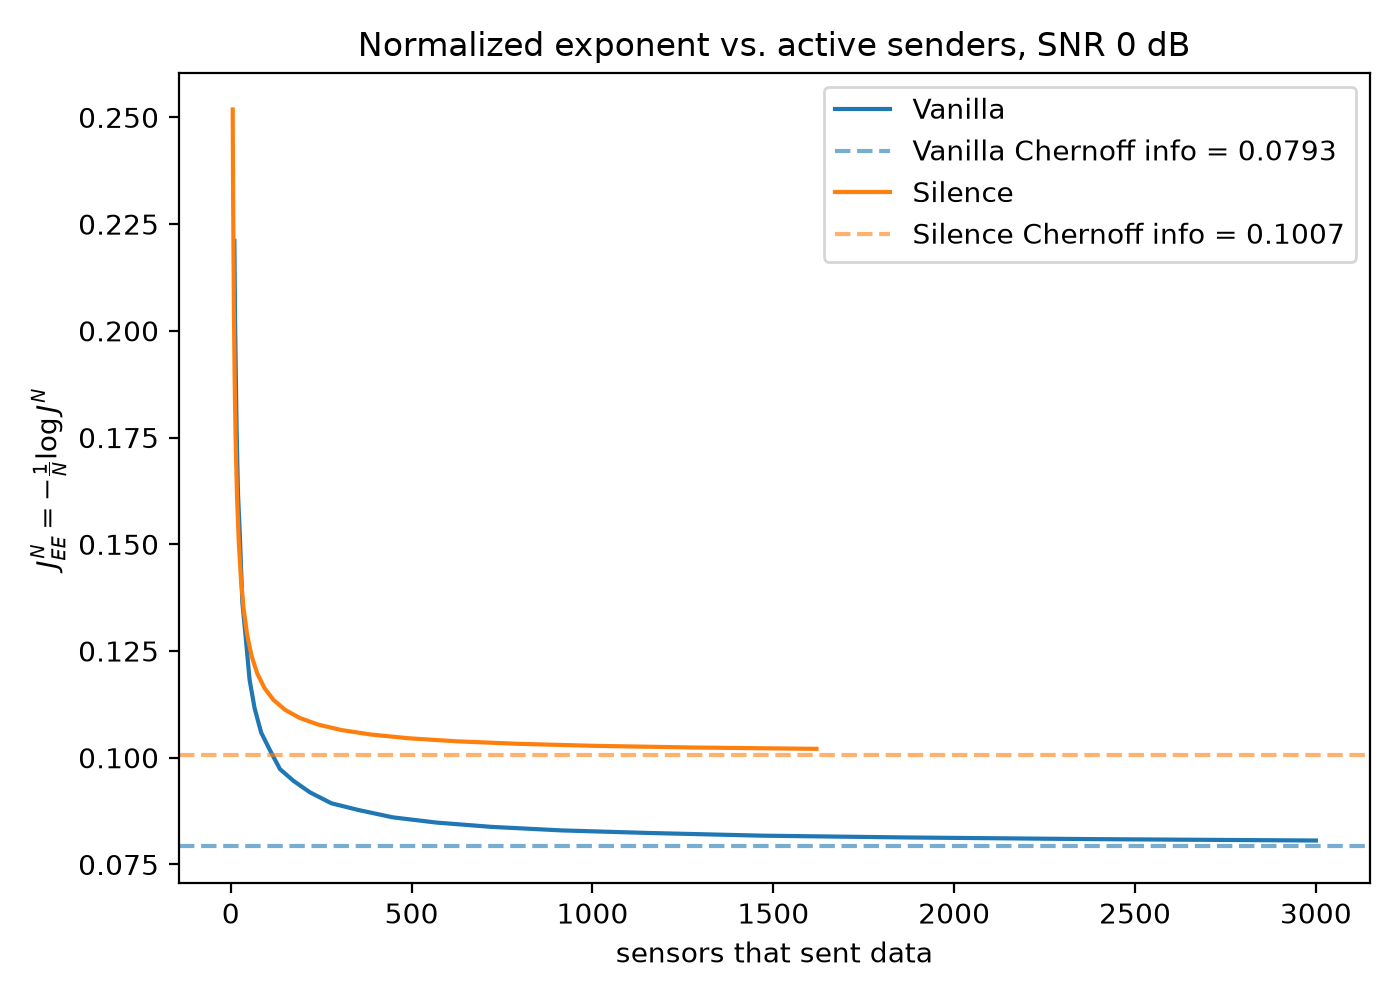
\includegraphics[width=0.65\textwidth]{Figs/fig_active_senders_normalized_chernoff.png}
%     \caption{Normalized error exponent $J^N_{EE}$ vs. number of active senders, SNR $= 0$~dB, for the vanilla and silent policies, with their Chernoff-information asymptotes $C_V \approx 0.0793$ and $C_S \approx 0.1007$ shown as dashed lines.}
%     \label{fig:active-senders-chernoff}
% \end{figure}


\newpage

\section{Appendix}
\subsection{Full Derivation of the Error Exponent}
\label{app:error-exponent}
\subsubsection*{Error I - $P(\gamma^0(u^{0:N}) = 1|H_2)$}
Recalling that the optimal decision rule dictates that $\gamma^0(u^{0:N}) = 1$ if:
\begin{align}
    \sum_{i=1}^{N}\log\frac{P^{\gamma^i}(u^i|H_1)}{P^{\gamma^i}(u^i|H_2)} > Nt
\end{align}
Applying the Chernoff bound with $\alpha > 0$:
\begin{align}
    P(\gamma^0(u^{0:N}) = 1|H_2) = P\bigg(\sum_{i=1}^{N}\log\frac{P^{\gamma^i}(u^i|H_1)}{P^{\gamma^i}(u^i|H_2)} > Nt\bigg|H_2\bigg) \leq E_{H_2}\bigg[\exp\bigg(\alpha \sum_{i=1}^{N}\log\frac{P^{\gamma^i}(u^i|H_1)}{P^{\gamma^i}(u^i|H_2)}\bigg)\bigg]e^{-\alpha Nt}
\end{align}
From the independence of $y^i|H$:
\begin{align}
    E_{H_2}\bigg[\exp\bigg(\alpha \sum_{i=1}^{N}\log\frac{P^{\gamma^i}(u^i|H_1)}{P^{\gamma^i}(u^i|H_2)}\bigg)\bigg] = \prod_{i=1}^{N}E_{H_2}\bigg[\exp\bigg(\alpha \log\frac{P^{\gamma^i}(u^i|H_1)}{P^{\gamma^i}(u^i|H_2)}\bigg)\bigg] = \prod_{i=1}^{N}E_{H_2}\bigg[\bigg(\frac{P^{\gamma^i}(u^i|H_1)}{P^{\gamma^i}(u^i|H_2)}\bigg)^\alpha\bigg]
\end{align}
We can calculate a single expectation:
\begin{align}
    E_{H_2}\bigg[\bigg(\frac{P^{\gamma^i}(u^i|H_1)}{P^{\gamma^i}(u^i|H_2)}\bigg)^\alpha\bigg] = \sum_{u \in \mathcal{U}} P^{\gamma^i}(u^i|H_2)\bigg(\frac{P^{\gamma^i}(u^i|H_1)}{P^{\gamma^i}(u^i|H_2)}\bigg)^\alpha = \sum_{u \in \mathcal{U}} P^{\gamma^i}(u^i|H_2)^{1-\alpha}P^{\gamma^i}(u^i|H_1)^{\alpha}
\end{align}
We now define the policy-dependent Chernoff coefficient $M(\alpha,\gamma^i) \triangleq \sum_{u \in \mathcal{U}} P^{\gamma^i}(u^i|H_2)^{1-\alpha}P^{\gamma^i}(u^i|H_1)^{\alpha}$, the probability of Error I is bound by:
\begin{align}
    P(\gamma^0(u^{0:N}) = 1|H_2) \leq \prod_{i=1}^{N}M(\alpha,\gamma^i)e^{-\alpha Nt}
\end{align}

\subsubsection*{Error II - $P(\gamma^0(u^{0:N}) = 2|H_1)$}
In a similar manner, $\gamma^0(u^{0:N}) = 2$ if:
\begin{align}
    \sum_{i=1}^{N}\log\frac{P^{\gamma^i}(u^i|H_1)}{P^{\gamma^i}(u^i|H_2)} < Nt \iff -\sum_{i=1}^{N}\log\frac{P^{\gamma^i}(u^i|H_1)}{P^{\gamma^i}(u^i|H_2)} > -Nt
\end{align}
Applying the Chernoff bound with $\beta > 0$:
\begin{align}
    P(\gamma^0(u^{0:N}) = 2|H_1) = P\bigg(-\sum_{i=1}^{N}\log\frac{P^{\gamma^i}(u^i|H_1)}{P^{\gamma^i}(u^i|H_2)} > -Nt\bigg|H_1\bigg) \leq E_{H_1}\bigg[\exp\bigg(-\beta \sum_{i=1}^{N}\log\frac{P^{\gamma^i}(u^i|H_1)}{P^{\gamma^i}(u^i|H_2)}\bigg)\bigg]e^{\beta Nt}
\end{align}
To align our results, we demand $\beta = 1-\alpha$, resulting in $\alpha < 1$. From the independence of $y^i|H$:
\begin{align}
    E_{H_1}\bigg[\exp\bigg(-\beta \sum_{i=1}^{N}\log\frac{P^{\gamma^i}(u^i|H_1)}{P^{\gamma^i}(u^i|H_2)}\bigg)\bigg] = \prod_{i=1}^{N}E_{H_1}\bigg[\bigg(\frac{P^{\gamma^i}(u^i|H_1)}{P^{\gamma^i}(u^i|H_2)}\bigg)^{(\alpha-1)}\bigg]
\end{align}
The expectation:
\begin{align}
    E_{H_1}\bigg[\bigg(\frac{P^{\gamma^i}(u^i|H_1)}{P^{\gamma^i}(u^i|H_2)}\bigg)^{(\alpha - 1)}\bigg] &= \sum_{u \in \mathcal{U}}P^{\gamma^i}(u^i|H_1)\bigg(\frac{P^{\gamma^i}(u^i|H_1)}{P^{\gamma^i}(u^i|H_2)}\bigg)^{(\alpha - 1)} \\
    &= \sum_{u \in \mathcal{U}} P^{\gamma^i}(u^i|H_2)^{1-\alpha}P^{\gamma^i}(u^i|H_1)^{\alpha} = M(\alpha,\gamma^i)
\end{align}
The resulting bound for Error II is:
\begin{align*}
    P(\gamma^0(u^{0:N}) = 2|H_1) \leq \prod_{i=1}^{N}M(\alpha,\gamma^i)e^{(1-\alpha)Nt}
\end{align*}

\subsubsection*{Error probability bound}
The probability of error is $P_e = (1-p)\cdot P(\gamma^0(u^{0:N}) = 1|H_2) + p\cdot P(\gamma^0(u^{0:N}) = 2|H_1)$, applying the bounds:
\begin{align}
    P_e \leq (1-p)\cdot \prod_{i=1}^{N}M(\alpha,\gamma^i)e^{-\alpha Nt} + p\cdot \prod_{i=1}^{N}M(\alpha,\gamma^i)e^{(1-\alpha) Nt}\\
    = e^{-\alpha Nt}\bigg((1-p) + pe^{Nt}\bigg) \prod_{i=1}^{N}M(\alpha,\gamma^i)\\
    = (\frac{p}{1-p})^\alpha\cdot2(1-p)\prod_{i=1}^{N}M(\alpha,\gamma^i)\\
    =2\cdot p^\alpha \cdot (1-p)^{1-\alpha}\prod_{i=1}^{N}M(\alpha,\gamma^i)
\end{align}
Recalling that $Nt = \log\frac{1-p}{p}$ yields $e^{-\alpha Nt} = (\frac{p}{1-p})^\alpha$ and $e^{Nt} = (\frac{1-p}{p})$, and $\alpha \in [0,1]$.

\subsubsection*{Error Exponent}
Recalling the discussion in Section~\ref{sec:exp-decay}, we can now bound the error exponent:

\begin{align}
    \JNEE  = -\frac{1}{N}\log(P_e) \geq -\frac{1}{N}\log(2) -\frac{1}{N}\log(p^\alpha (1-p)^{1-\alpha})-\frac{1}{N}\log\bigg( \prod_{i=1}^{N}M(\alpha,\gamma^i) \bigg)
\end{align}

Taking the limit will cause the constants to vanish resulting in:

\begin{align}
    \lim_{N \to \infty}\JNEE &\geq\lim_{N \to \infty} -\frac{1}{N}\log\bigg( \prod_{i=1}^{N}M(\alpha,\gamma^i) \bigg)\\
    &= \lim_{N \to \infty} -\frac{1}{N}\sum_{i=1}^{N} \log(M(\alpha,\gamma^i))
\end{align}
Assuming there are $K$ different policies, and $N_k$ sensors using each, meaning $\sum_{k=1}^{K}N_k = N$.\\
Define $\lim_{N \to \infty}\frac{N_k}{N} \triangleq c_k$ we get:
\begin{align}
    \lim_{N \to \infty}\JNEE \geq -\min_{\alpha \in [0,1]}\sum_{k=1}^{K} c_k \log M(\alpha,\gamma^k)
\end{align}

\subsection{Vanilla Policy: Full Threshold and Chernoff Coefficient Derivation}
\label{app:vanilla-derivation}
We first derive the decision threshold for the vanilla setup used in Section~\ref{sec:considering-rate}. By Lemma 1, the optimal decision rule is a threshold $\tau$ on the likelihood ratio: the sensor transmits $u^2$ if
\begin{align*}
    L(y) = \frac{f_{y|H_2}(y|H_2)}{f_{y|H_1}(y|H_1)} \geq \tau
\end{align*}
and $u^1$ otherwise. Under the Gaussian assumption, $L(y)$ simplifies to
\begin{align*}
    L(y) = \frac{f_{y|H_2}(y|H_2)}{f_{y|H_1}(y|H_1)} = \exp\bigg(\frac{-(y-\mu)^2 + y^2}{2\sigma^2}\bigg) = \exp\bigg(\frac{2y\mu-\mu^2}{2\sigma^2}\bigg)
\end{align*}
Taking $\log$ gives the log-likelihood ratio
\begin{align*}
    \log(L(y)) = \frac{y\mu}{\sigma^2} - \frac{\mu^2}{2\sigma^2} &\geq \log(\tau) \\
    \frac{y\mu}{\sigma^2} &\geq \log(\tau) + \frac{\mu^2}{2\sigma^2}\\
    y &\geq \frac{\sigma^2}{\mu}\log(\tau) + \frac{\mu}{2} \triangleq \lambda_V
\end{align*}
Since the optimal rule corresponds to $\tau = 1$, this reduces to a threshold on $y$ at $\lambda_V = \frac{\mu}{2}$, as used in Section~\ref{sec:considering-rate}.

We now compute the Chernoff coefficient of the vanilla policy:
\begin{align}
    &M_{V}(\alpha,\gamma^V) = P^{\gamma^V}(u^1|H_1)^\alpha \cdot P^{\gamma^V}(u^1|H_2)^{1-\alpha} + P^{\gamma^V}(u^2|H_1)^\alpha \cdot P^{\gamma^V}(u^2|H_2)^{1-\alpha}\\
    &M_{V}(\alpha) = Q(\frac{\mu}{2\sigma})^{\alpha} \cdot (1-Q(\frac{\mu}{2\sigma}))^{1-\alpha} + Q(\frac{\mu}{2\sigma})^{1-\alpha} \cdot (1-Q(\frac{\mu}{2\sigma}))^{\alpha}
\end{align}
Since $M_V(\alpha) = M_V(1-\alpha)$, $M_V$ is symmetric about $\alpha = 0.5$; together with its convexity on $[0,1]$, this means $M_V$ attains its minimum at $\alpha = 0.5$, giving
\begin{align}
    \JNEE \geq -\min_{\alpha\in[0,1]}\log M_{V}(\alpha) = -\log\bigg(2 \sqrt{Q(\frac{\mu}{2\sigma}) \cdot (1-Q(\frac{\mu}{2\sigma}))}\bigg)
\end{align}
This is the Chernoff distance bound for the vanilla policy, quoted in Section~\ref{sec:considering-rate}.

\subsection{Silent Policy: Full Threshold and Chernoff Coefficient Derivation}
\label{app:silent-derivation}
Recall the silent setup of Section~\ref{sec:considering-rate}. We introduce two thresholds $\tau_1 < \tau_2$ on the likelihood ratio: the sensor sends $u^1$ if $L(y) < \tau_1$, $u^2$ if $L(y) > \tau_2$, and stays silent ($u^S$) otherwise:
\begin{align*}
    R_1 = \{y \in \mathcal{Y}: L(y) < \tau_1\}, \quad R_S = \{y \in \mathcal{Y}: \tau_1 \leq L(y) \leq \tau_2\}, \quad R_2 = \{y \in \mathcal{Y}: L(y) > \tau_2\}
\end{align*}
Since $L(y)$ is increasing in $y$ (Appendix~\ref{app:vanilla-derivation}), these map to thresholds on $y$: with $\lambda_i \triangleq \frac{\sigma^2}{\mu}\log(\tau_i) + \frac{\mu}{2}$ for $i=1,2$ and $\lambda_1 < \lambda_2$,
\begin{align*}
    R_1 = \{y < \lambda_1\}, \quad R_S = \{\lambda_1 \leq y \leq \lambda_2\}, \quad R_2 = \{y > \lambda_2\}
\end{align*}
giving the decision rule $\gamma^S$:
\begin{itemize}
    \item $P^{\gamma^S}(u^1|H_j) = \int_{R_1}f_{y|H_j}(y|H_j)dy$
    \item $P^{\gamma^S}(u^S|H_j) = \int_{R_S}f_{y|H_j}(y|H_j)dy$
    \item $P^{\gamma^S}(u^2|H_j) = \int_{R_2}f_{y|H_j}(y|H_j)dy$
\end{itemize}
Evaluating these integrals under the Gaussian model gives:
\begin{itemize}
    \item $P(u^1|H_1) = P(y<\lambda_1|H_1) = 1-Q(\frac{\lambda_1}{\sigma})$
    \item $P(u^S|H_1) = P(\lambda_1\leq y\leq\lambda_2|H_1) = Q(\frac{\lambda_1}{\sigma}) - Q(\frac{\lambda_2}{\sigma})$
    \item $P(u^2|H_1) = P(y>\lambda_2|H_1) = Q(\frac{\lambda_2}{\sigma})$
    \item $P(u^1|H_2) = P(y<\lambda_1|H_2) = 1-Q(\frac{\lambda_1-\mu}{\sigma})$
    \item $P(u^S|H_2) = P(\lambda_1\leq y\leq\lambda_2|H_2) = Q(\frac{\lambda_1-\mu}{\sigma}) - Q(\frac{\lambda_2-\mu}{\sigma})$
    \item $P(u^2|H_2) = P(y>\lambda_2|H_2) = Q(\frac{\lambda_2-\mu}{\sigma})$
\end{itemize}
$\lambda_1$ and $\lambda_2$ are in general independent, but since the two Gaussians share variance $\sigma^2$ and differ only in mean, the optimal boundaries are symmetric about the midpoint $\frac{\mu}{2}$. We therefore parametrize them by a single variable $\delta > 0$:
\begin{align*}
    \lambda_1 = \frac{\mu}{2} - \delta, \qquad \lambda_2 = \frac{\mu}{2} + \delta
\end{align*}
reducing the optimization to a single free parameter. Denoting
\begin{align*}
    q_+ \triangleq Q\Big(\frac{\mu/2+\delta}{\sigma}\Big), \qquad q_- \triangleq Q\Big(\frac{\mu/2-\delta}{\sigma}\Big)
\end{align*}
and substituting $\lambda_1,\lambda_2$ into the probabilities above gives:
\begin{itemize}
    \item $P(u^1|H_1) = 1-q_-, \quad P(u^S|H_1) = q_- - q_+, \quad P(u^2|H_1) = q_+$
    \item $P(u^1|H_2) = q_+, \quad P(u^S|H_2) = q_- - q_+, \quad P(u^2|H_2) = 1-q_-$
\end{itemize}
as used in Section~\ref{sec:considering-rate}. We now compute the Chernoff coefficient of the silent policy:
\begin{align}
    &M_{S}(\alpha,\gamma^S) = P^{\gamma^S}(u^1|H_1)^\alpha P^{\gamma^S}(u^1|H_2)^{1-\alpha} + P^{\gamma^S}(u^S|H_1)^\alpha P^{\gamma^S}(u^S|H_2)^{1-\alpha}\\
    &\qquad + P^{\gamma^S}(u^2|H_1)^\alpha P^{\gamma^S}(u^2|H_2)^{1-\alpha}\\
    &M_{S}(\alpha) = (1-q_-)^{\alpha}q_+^{1-\alpha} + (q_--q_+)^{\alpha}(q_--q_+)^{1-\alpha} + q_+^{\alpha}(1-q_-)^{1-\alpha}
\end{align}
Since $P(u^S|H_1) = P(u^S|H_2) = q_--q_+$, the middle term collapses to $q_--q_+$ regardless of $\alpha$:
\begin{align}
    M_{S}(\alpha) = (q_--q_+) + (1-q_-)^{\alpha}q_+^{1-\alpha} + q_+^{\alpha}(1-q_-)^{1-\alpha}
\end{align}
Swapping $\alpha \leftrightarrow 1-\alpha$ leaves the constant term unchanged and exchanges the remaining two, so $M_S(\alpha) = M_S(1-\alpha)$; together with convexity on $[0,1]$, this means $M_S$ attains its minimum at $\alpha = 0.5$, as in the vanilla case, giving
\begin{align}
    \JNEE \geq -\min_{\alpha\in[0,1]}\log M_{S}(\alpha) = -\log\Big((q_--q_+) + 2\sqrt{(1-q_-)q_+}\Big)
\end{align}
This is the Chernoff distance bound for the silent policy, quoted in Section~\ref{sec:considering-rate}.

\subsection{Optimal Silence Threshold}
\label{app:delta}
\paragraph{The objective.} Substituting $q_\pm = Q\big(\frac{\mu/2\pm\delta}{\sigma}\big)$ into Equation~\eqref{eq:MS-of-delta}:
\begin{equation}
    M_S(\delta) = \left[Q\Big(\frac{\mu/2-\delta}{\sigma}\Big) - Q\Big(\frac{\mu/2+\delta}{\sigma}\Big)\right] + 2\sqrt{\left[1-Q\Big(\frac{\mu/2-\delta}{\sigma}\Big)\right]Q\Big(\frac{\mu/2+\delta}{\sigma}\Big)}.
    \label{eq:MS-explicit}
\end{equation}
Using $1-Q(x) = Q(-x)$, equivalently
\begin{equation}
    M_S(\delta) = 1 - Q\Big(\frac{\delta-\mu/2}{\sigma}\Big) - Q\Big(\frac{\delta+\mu/2}{\sigma}\Big) + 2\sqrt{Q\Big(\frac{\delta-\mu/2}{\sigma}\Big)Q\Big(\frac{\delta+\mu/2}{\sigma}\Big)},
    \label{eq:MS-tails}
\end{equation}
giving $M_S(0) = 2\sqrt{q(1-q)} = M_V$ and $M_S(\delta)\to 1$ as $\delta\to\infty$.

\paragraph{Differentiation.} $Q(x) = \int_x^\infty \frac{1}{\sqrt{2\pi}}e^{-t^2/2}dt$, so $Q'(x) = -\phi(x)$ with $\phi(x) = \frac{1}{\sqrt{2\pi}}e^{-x^2/2}$. The inner derivatives are $\mp 1/\sigma$, so
\begin{equation}
    \frac{d}{d\delta}\left[Q\Big(\frac{\mu/2-\delta}{\sigma}\Big) - Q\Big(\frac{\mu/2+\delta}{\sigma}\Big)\right] = \frac{1}{\sigma}\left[\phi\Big(\frac{\mu/2-\delta}{\sigma}\Big) + \phi\Big(\frac{\mu/2+\delta}{\sigma}\Big)\right].
\end{equation}
For $f(\delta) \triangleq \left[1-Q\Big(\frac{\mu/2-\delta}{\sigma}\Big)\right]Q\Big(\frac{\mu/2+\delta}{\sigma}\Big)$,
\begin{equation}
    f'(\delta) = -\frac{1}{\sigma}\phi\Big(\frac{\mu/2-\delta}{\sigma}\Big)Q\Big(\frac{\mu/2+\delta}{\sigma}\Big) - \frac{1}{\sigma}\phi\Big(\frac{\mu/2+\delta}{\sigma}\Big)\left[1-Q\Big(\frac{\mu/2-\delta}{\sigma}\Big)\right],
\end{equation}
and $\frac{d}{d\delta}2\sqrt{f} = f'/\sqrt{f}$. Combining:
\begin{equation}
    \sigma\frac{dM_S}{d\delta} = \phi\Big(\frac{\mu/2-\delta}{\sigma}\Big) + \phi\Big(\frac{\mu/2+\delta}{\sigma}\Big) - \frac{\phi\Big(\frac{\mu/2-\delta}{\sigma}\Big)Q\Big(\frac{\mu/2+\delta}{\sigma}\Big) + \phi\Big(\frac{\mu/2+\delta}{\sigma}\Big)\left[1-Q\Big(\frac{\mu/2-\delta}{\sigma}\Big)\right]}{\sqrt{\left[1-Q\Big(\frac{\mu/2-\delta}{\sigma}\Big)\right]Q\Big(\frac{\mu/2+\delta}{\sigma}\Big)}},
    \label{eq:app-full-derivative}
\end{equation}
which is Equation~\eqref{eq:dMS} written out.

\paragraph{Factorization.} Multiplying by $AB>0$:
\begin{align}
    (\phi_-+\phi_+)AB - (\phi_-A^2+\phi_+B^2) &= \phi_-A(B-A) + \phi_+B(A-B) \nonumber\\
    &= (B-A)(\phi_-A-\phi_+B).
\end{align}
Since $B-A>0$, setting $M_S'=0$ forces $\phi_-A=\phi_+B$. The density ratio is closed form,
\begin{equation}
    \frac{\phi_-}{\phi_+} = \exp\left(\frac{(\mu/2+\delta)^2-(\mu/2-\delta)^2}{2\sigma^2}\right) = e^{\mu\delta/\sigma^2},
\end{equation}
which gives Equation~\eqref{eq:opt-delta}.

\begin{thebibliography}{9}

\bibitem{sanjari2025}
S.~Sanjari, N.~Saldi, S.~Gezici, and S.~Y\"uksel, ``Decentralized Detection with Many Sensors: Optimality of Exchangeable and Identical Encoding Policies,'' \emph{arXiv preprint arXiv:2509.21724}, Sep. 2025.

\bibitem{tsitsiklis1989}
J.~N.~Tsitsiklis, ``Decentralized Detection,'' Laboratory for Information and Decision Systems, Massachusetts Institute of Technology, Cambridge, MA, Tech. Rep. LIDS-P-1913, Sep. 1989. To appear in \emph{Advances in Statistical Signal Processing, Vol. 2: Signal Detection}, H.~V.~Poor and J.~B.~Thomas, Eds.

\bibitem{chernoff1952}
H.~Chernoff, ``A Measure of Asymptotic Efficiency for Tests of a Hypothesis Based on the Sum of Observations,'' \emph{Annals of Mathematical Statistics}, vol.~23, no.~4, pp.~493--507, Dec. 1952.

\end{thebibliography}

\end{document}
